\documentclass{article}
\usepackage[utf8]{inputenc}
\usepackage{float}
\usepackage[version=4]{mhchem}
\usepackage{natbib}
\usepackage{graphicx}
\usepackage{listings}
\usepackage{color}

\definecolor{dkgreen}{rgb}{0,0.6,0}
\definecolor{gray}{rgb}{0.5,0.5,0.5}
\definecolor{mauve}{rgb}{0.58,0,0.82}

\lstset{frame=tb,
  language=Python,
  aboveskip=3mm,
  belowskip=3mm,
  showstringspaces=false,
  columns=flexible,
  basicstyle={\small\ttfamily},
  numbers=none,
  numberstyle=\tiny\color{gray},
  keywordstyle=\color{blue},
  commentstyle=\color{dkgreen},
  stringstyle=\color{mauve},
  breaklines=true,
  breakatwhitespace=true,
  tabsize=3
}

\title{Computer Practicum 1}
\author{James Chen}
\date{March 2021}

\begin{document}

\maketitle

\section{First Reaction}
\begin{equation}
    \ce{A + B <=>T[k1][k-1] C}
\end{equation}
\begin{equation}
    \ce{C ->T[k2] D}
\end{equation}
\subsection{Zero Order}
\begin{figure}[H]
\centering
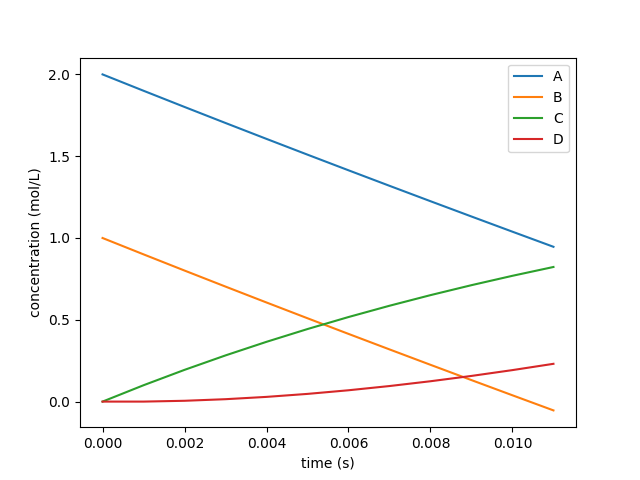
\includegraphics[scale=0.6]{1. zero.png}
\caption{Zero Order, \ce{[A]0}=2 \ce{[B]0}=1}
\end{figure}
As we can see from the graph that in zero order reaction, we cannot reach equilibrium,so steady-state approximation is not valid.

\subsection{First order}
\begin{figure}[H]
\centering
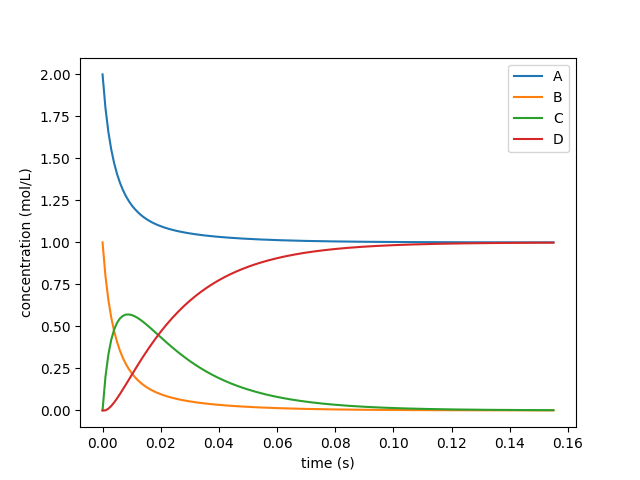
\includegraphics[scale=0.6]{1. first 2 1.png}
\caption{First Order, \ce{[A]0}=2 \ce{[B]0}=1}
\end{figure}
\begin{figure}[H]
\centering
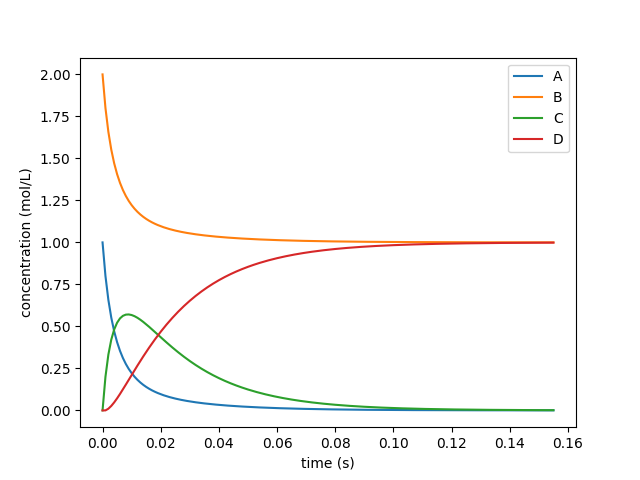
\includegraphics[scale=0.6]{1. first 1 2.png}
\caption{First Order, \ce{[A]0}=1 \ce{[B]0}=2}
\end{figure}
\begin{figure}[H]
\centering
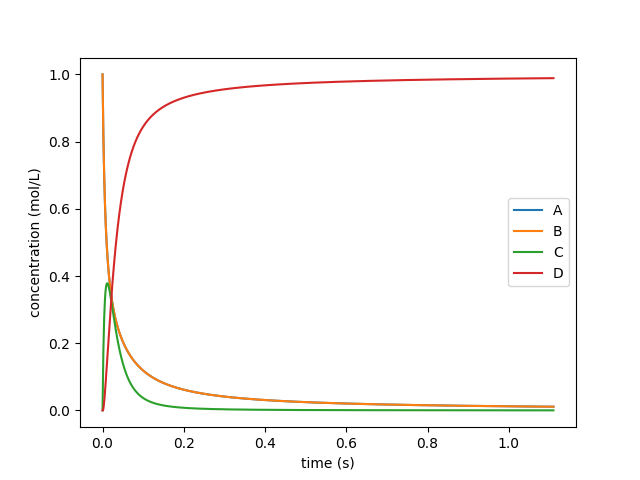
\includegraphics[scale=0.6]{1. first 1 1.png}
\caption{First Order, \ce{[A]0}=1 \ce{[B]0}=1}
\end{figure}
As we can see from the graphs that in first order reaction, we can reach equilibrium regardless of the initial concentration,so steady-state approximation is valid.


\section{Second Reaction ((The Enzyme Mechanisms)}
\begin{equation}
    \ce{A + B <=>T[k1][k-1] C}
\end{equation}
\begin{equation}
    \ce{C ->T[k2] D + A}
\end{equation}
\subsection{Zero Order}
\begin{figure}[H]
\centering
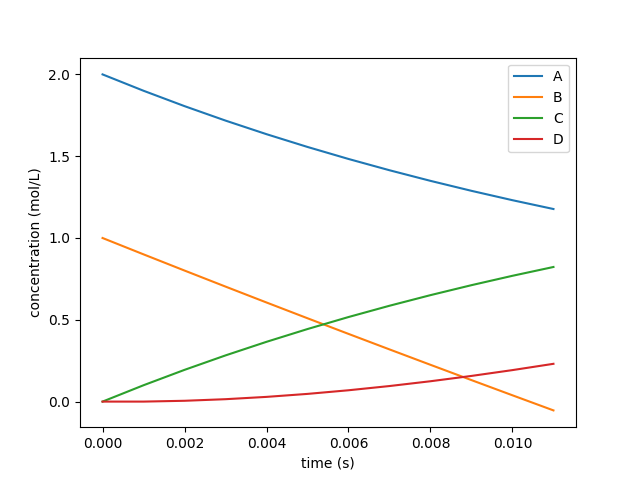
\includegraphics[scale=0.6]{2. zero.png}
\caption{Zero Order, \ce{[A]0}=2 \ce{[B]0}=1}
\end{figure}
As we can see from the graph that in zero order reaction, we cannot reach equilibrium,so steady-state approximation is not valid.

\subsection{First order}
\begin{figure}[H]
\centering
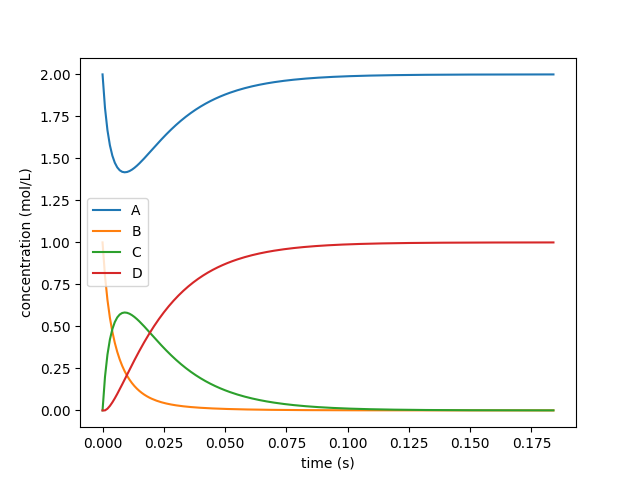
\includegraphics[scale=0.6]{2. first 2 1.png}
\caption{First Order, \ce{[A]0}=2 \ce{[B]0}=1}
\end{figure}
\begin{figure}[H]
\centering
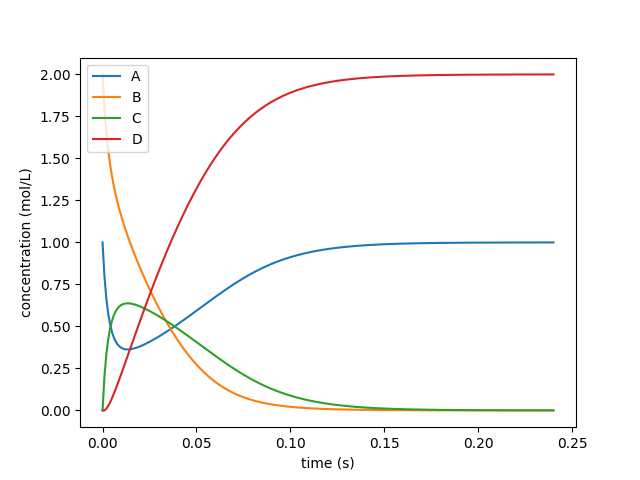
\includegraphics[scale=0.6]{2. first 1 2.png}
\caption{First Order, \ce{[A]0}=1 \ce{[B]0}=2}
\end{figure}
\begin{figure}[H]
\centering
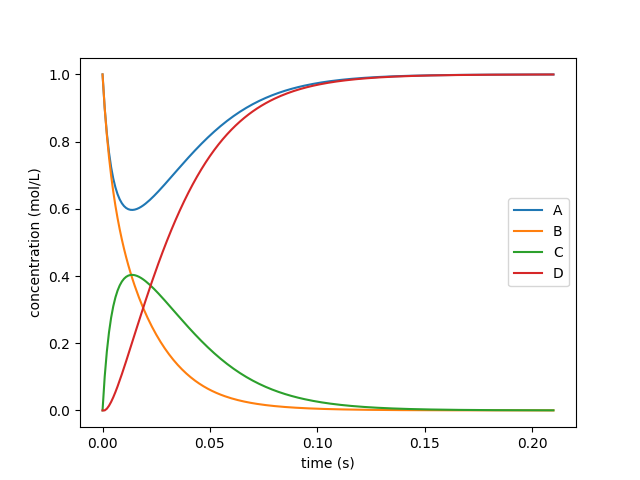
\includegraphics[scale=0.6]{2. first 1 1.png}
\caption{First Order, \ce{[A]0}=1 \ce{[B]0}=1}
\end{figure}
As we can see from the graphs that in first order reaction, we can reach equilibrium regardless of the initial concentration,so steady-state approximation is valid.

\newpage
\section*{Appendix I: Python Code For First Reaction}
\begin{lstlisting}
import matplotlib.pyplot as plt 
#def rate constant k and initial concentration
k1f = 100
k1r = 10
k2 = 50
A = 1
B = 1
C = 0
D = 0
#set rate order
oa = 1
ob = 1
#def time slot
time = 0
time_slot = 1e-3
#Crate lists
A_list = [A]
B_list = [B]
C_list = [C]
D_list = [D]
time_list = [time]
#Begin compute and mark the following points
loop = True
while loop:
    time = time + time_slot
    print("current reaction time:", time)
    # compute slope
    slopeA = -k1f * (A**oa) * (B**ob) + k1r * C
    slopeB = -k1f * (A**oa) * (B**ob) + k1r * C
    slopeC = k1f * (A**oa) * (B**ob) -k1r * C - k2 * C
    slopeD = k2 * C
    # compute concentration
    A = A + slopeA * time_slot
    B = B + slopeB * time_slot
    C = C + slopeC * time_slot
    D = D + slopeD * time_slot
    # add to lists
    A_list += [A]
    B_list += [B]
    C_list += [C]
    D_list += [D]
    time_list += [time]
    # test if reaches convergence
    if slopeA >= 1e-2 or slopeA<= -1e-2:
        loop  =True
    else:
        loop = False
    if oa ==0 and ob ==0:
        if A < 0 or B < 0 or C < 0 or D < 0:
            loop = False
#fig info
plt.plot(time_list, A_list, label = "A")
plt.plot(time_list, B_list, label = "B")
plt.plot(time_list, C_list, label = "C")
plt.plot(time_list, D_list, label = "D")
plt.legend(['A', 'B', 'C', 'D'])
plt.ylabel("concentration (mol/L)")
plt.xlabel("time (s)")
plt.savefig('reaction sim.png')
plt.show()
\end{lstlisting}

\newpage
\section*{Appendix II: Python Code For Second Reaction}
\begin{lstlisting}
import matplotlib.pyplot as plt 
#def rate constant k and initial concentration
k1f = 100
k1r = 10
k2 = 50
A = 1
B = 1
C = 0
D = 0
#set rate order
oa = 1
ob = 1
#def time slot
time = 0
time_slot = 1e-3
#Crate lists
A_list = [A]
B_list = [B]
C_list = [C]
D_list = [D]
time_list = [time]
#Begin compute and mark the following points
loop = True
while loop:
    time = time + time_slot
    print("current reaction time:", time)
    # compute slope
    slopeA = -k1f * (A**oa) * (B**ob) + k1r * C + k2 * C
    slopeB = -k1f * (A**oa) * (B**ob) + k1r * C
    slopeC = k1f * (A**oa) * (B**ob) -k1r * C - k2 * C
    slopeD = k2 * C
    # compute concentration
    A = A + slopeA * time_slot
    B = B + slopeB * time_slot
    C = C + slopeC * time_slot
    D = D + slopeD * time_slot
    # add to lists
    A_list += [A]
    B_list += [B]
    C_list += [C]
    D_list += [D]
    time_list += [time]
    # test if reaches convergence
    if slopeA >= 1e-2 or slopeA<= -1e-2:
        loop  =True
    else:
        loop = False
    if oa ==0 and ob ==0:
        if A < 0 or B < 0 or C < 0 or D < 0:
            loop = False
#fig info
plt.plot(time_list, A_list, label = "A")
plt.plot(time_list, B_list, label = "B")
plt.plot(time_list, C_list, label = "C")
plt.plot(time_list, D_list, label = "D")
plt.legend(['A', 'B', 'C', 'D'])
plt.ylabel("concentration (mol/L)")
plt.xlabel("time (s)")
plt.savefig('reaction sim 2.png')
plt.show()
\end{lstlisting}


\end{document}
